\begin{savequote}[8cm]

	"I've made peace with myself."\newline
	"Good for you. That's the hardest war of all to win."\newline
	"Didn't say I won. Just stopped fighting."\newline
	\qauthor{―-- Joe Abercrombie, \textit{Best Served Cold}}
\end{savequote}

\chapter{Conclusion}

With a year-over-year increase in the amount of publicly available \gls{ngs} data, there is a need for machine learning methods to interpret biologically meaningful patterns and generate hypotheses for further study. This thesis introduces two new methods, SMCSMC and BLDA. I use these two new methods to analyse existing NGS data and draw novel conclusions about human history and the regulatory landscape of MLL-AF4 leukemia respectively. In this chapter, I discuss the implications of both the methods developed and the results generated. I finish with a statement on the overall applicability of machine learning to sequencing data and what I believe to be fruitful directions for further study.  

\section{Extending the SMC2 particle filter}

Inferring the \gls{arg} from a sample of individuals has been a longstanding goal in population genetics. Recently, four approaches have been developed that directly tackle this problem using modern methodologies and data. The \gls{smc2} method, introduced in \textcite{10.1371/journal.pone.0247647} with further exposition in this thesis, is unique in its ability to infer time-dependant directional migration rates due to its ``first-class'' treatment of migration as a distinct node in each marginal tree. Though this is certainly an attractive property of the algorithm, its distinct and incredibly flexible implementation can allow for the inference of essentially any process which admits simulation along the sequence. This includes, for example, background selection. This process of reducing a loci's diversity as a consequence of linkage with selected alleles has the potential to directly impact demographic inference due to the general assumption of selective neutrality. \textcite{Johri2021} starkly demonstrate this principle with regards to MSMC and \textit{fastsimcoal2} and there is no reason why SMC2 would fare better in these comparisons. With modifications of the \gls{cwr} which allow for the simulation of purifying selection (e.g. \cite{Zeng2012}) and unifying programs for performing population genetics simulations such as \textcite{Adrion2020a}, inference from a sample of ARGs generated with the particle filter could be expanded to include additional parameters for selection. 

Increasing the number of populations in the model would also massively increase its applicability to real world problems. This is possible with the method as it is, though the implementation would be non-trivial. In my opinion, this and other related problems could be solved by incorporating a standard backend solution for simulating and storing ARGs such as tskit (\url{https://github.com/tskit-dev/tskit}). Along with reducing the computational task of implementing different simulation models on the back ends, this would provide interoperability with the current gold-standard format for inferred ARGs. I have made preliminary efforts in this direction by providing a script to convert a sample of the inferred ARGs to the tskit format (and \textcite{Speidel2019a} have done the same), however issues with compatibility between the encoding of migration nodes in SMC2's trees has limited the usefulness of this approach. 

Another beneficial implementation-specific extension would be offloading computationally expensive steps to a graphical processing unit (GPU) implementation of a particle filter. Recent work has shown incredible computational gains in time-sensitive industrial applications such as robotics and manufacturing on the order of 10x runtime improvements simply by switching architectures \cite{Gelencser-Horvath2013,Murray2012,Lopez2015a}. As SMC2 is an asymptotically exact inference procedure in the limit of compute time, performing 10x the iterations in the same amount of time would improve (i) the resolution of existing analyses, (ii) the ability to infer from a larger number of haplotypes, (iii) the ability to infer a larger number of populations as stated above, and (iv) the ability to infer more recent events than 10 kya. Though this represents a significant amount of opportunity cost in terms of the time spent implementing the algorithm within the context of GPU libraries, the particle filter methodology is an excellent fit for many problems in population genetics and significantly speeding up the inference procedure would greatly simplify many outstanding problems in the field. 

\section{An ancestral back-migration in the context of African pre-history}

In Chapter 2, I applied SMC2 to two databases of global genetic variation and detected a large surplus of directional migration from populations deriving from the \gls{ooa} migration event backwards to those still living in Africa. The observation of this event is not unprecedented, as explored in the Discussion section of that chapter, however the data from single-tree inference in Y chromosome and \gls{mtDNA} is only able to state lower-bounds on the timing and is completely unable to estimate the proportion of the genome impacted. Since posting the study as a preprint on bioArxiv, two independent groups (\textcite{Montinaro2020,Wang2021}) have replicated our findings. Replication with independent methodologies lends confidence as to the robustness of the results. The estimates of magnitude from SMC2 are imprecise as demonstrated by simulation, however we expect a large scale back migration to become a commonly modelled feature of African pre-history in future demographic simulations. 

One of the most interesting questions arising from this investigation is the identity of the participants in the migration. One suggestion is that the participants may be descended from the unobserved ancestral basal Eurasian branch. These individuals are theorized to have diverged from the \gls{ooa} population around the same time as Neanderthal admixture was taking place approximately 55 kya before contributing to several Western Eurasian lineages \cite{Lazaridis2016,Lazaridis2018}. This would explain the lack of similarity that we see in the isolated segments to Neanderthals, despite their putatively Eurasian identity, and line up well with the assumed timeline of the migration. The actual dynamics of the migration itself is better phrased as an anthropological or archaeological question, and fine-tuning the resolution of the timing, magnitude, and participants aside, an inter-disciplinary approach will be fruitful when investigating this event in the future.


\begin{figure}
	\centering
	\subcaptionbox{Ju hoan North}{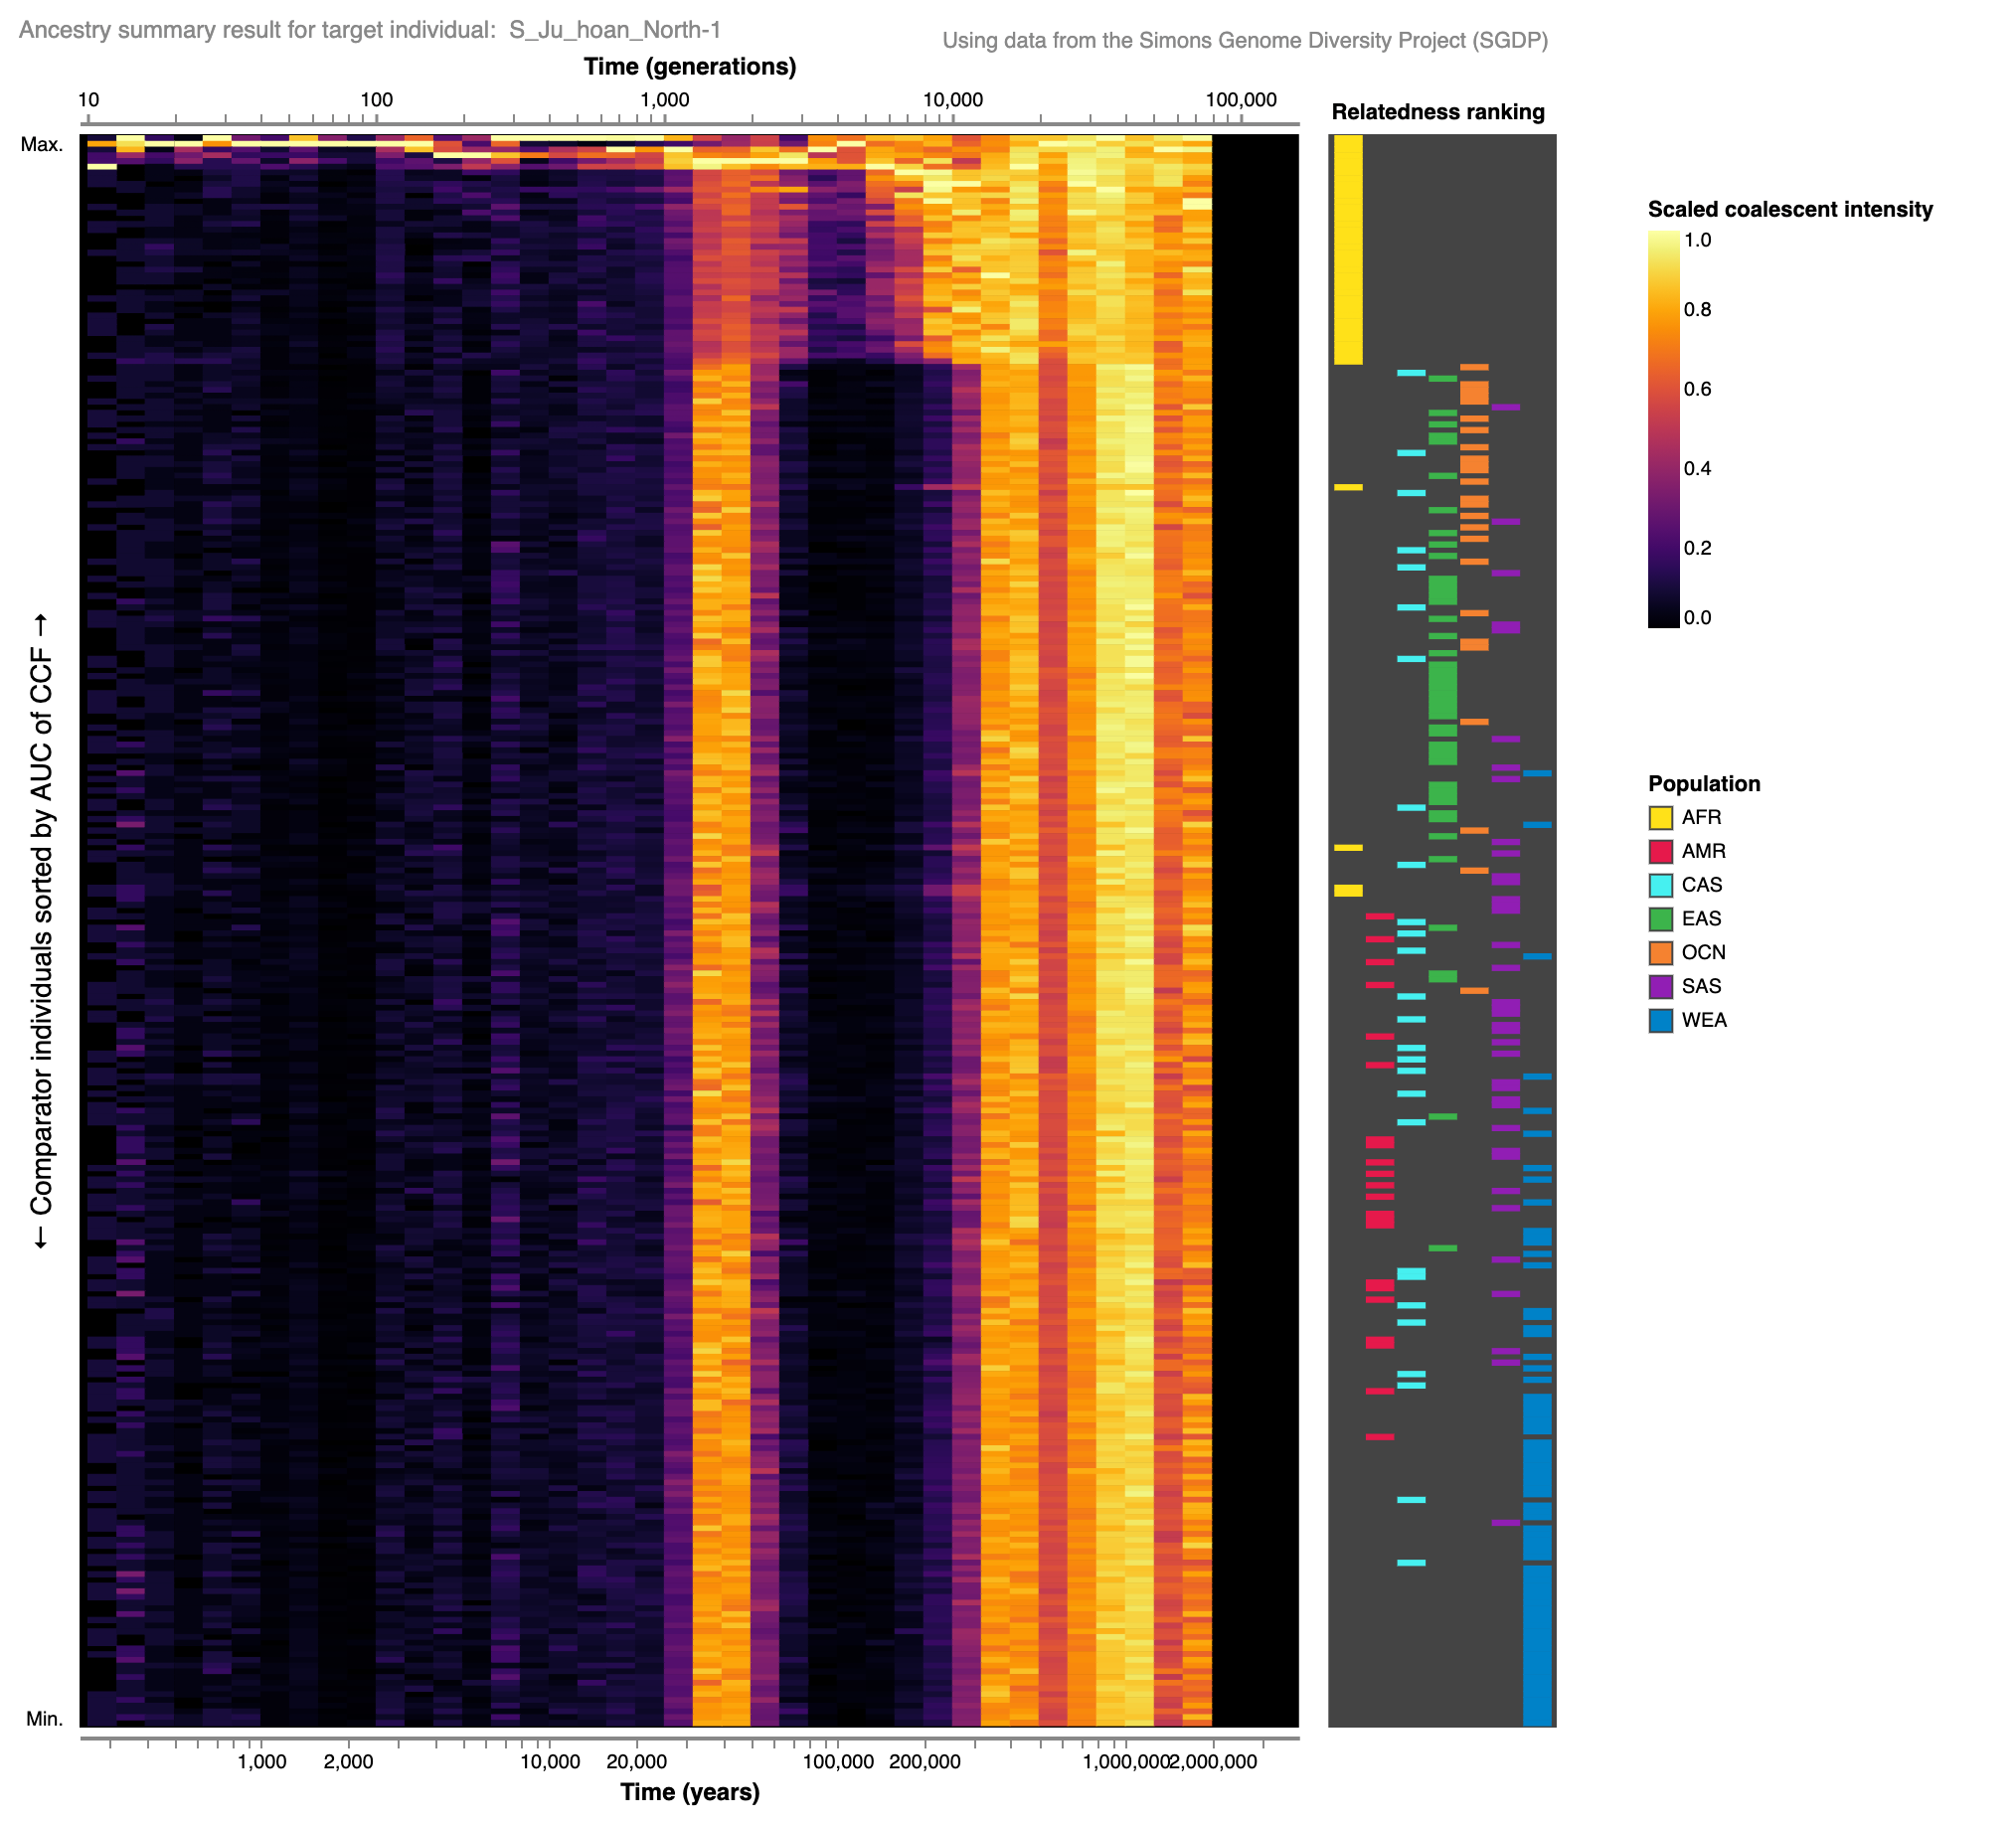
\includegraphics[width=0.5\textwidth]{plot/ch6/san}}%
	\hfill
	\subcaptionbox{Luhya}{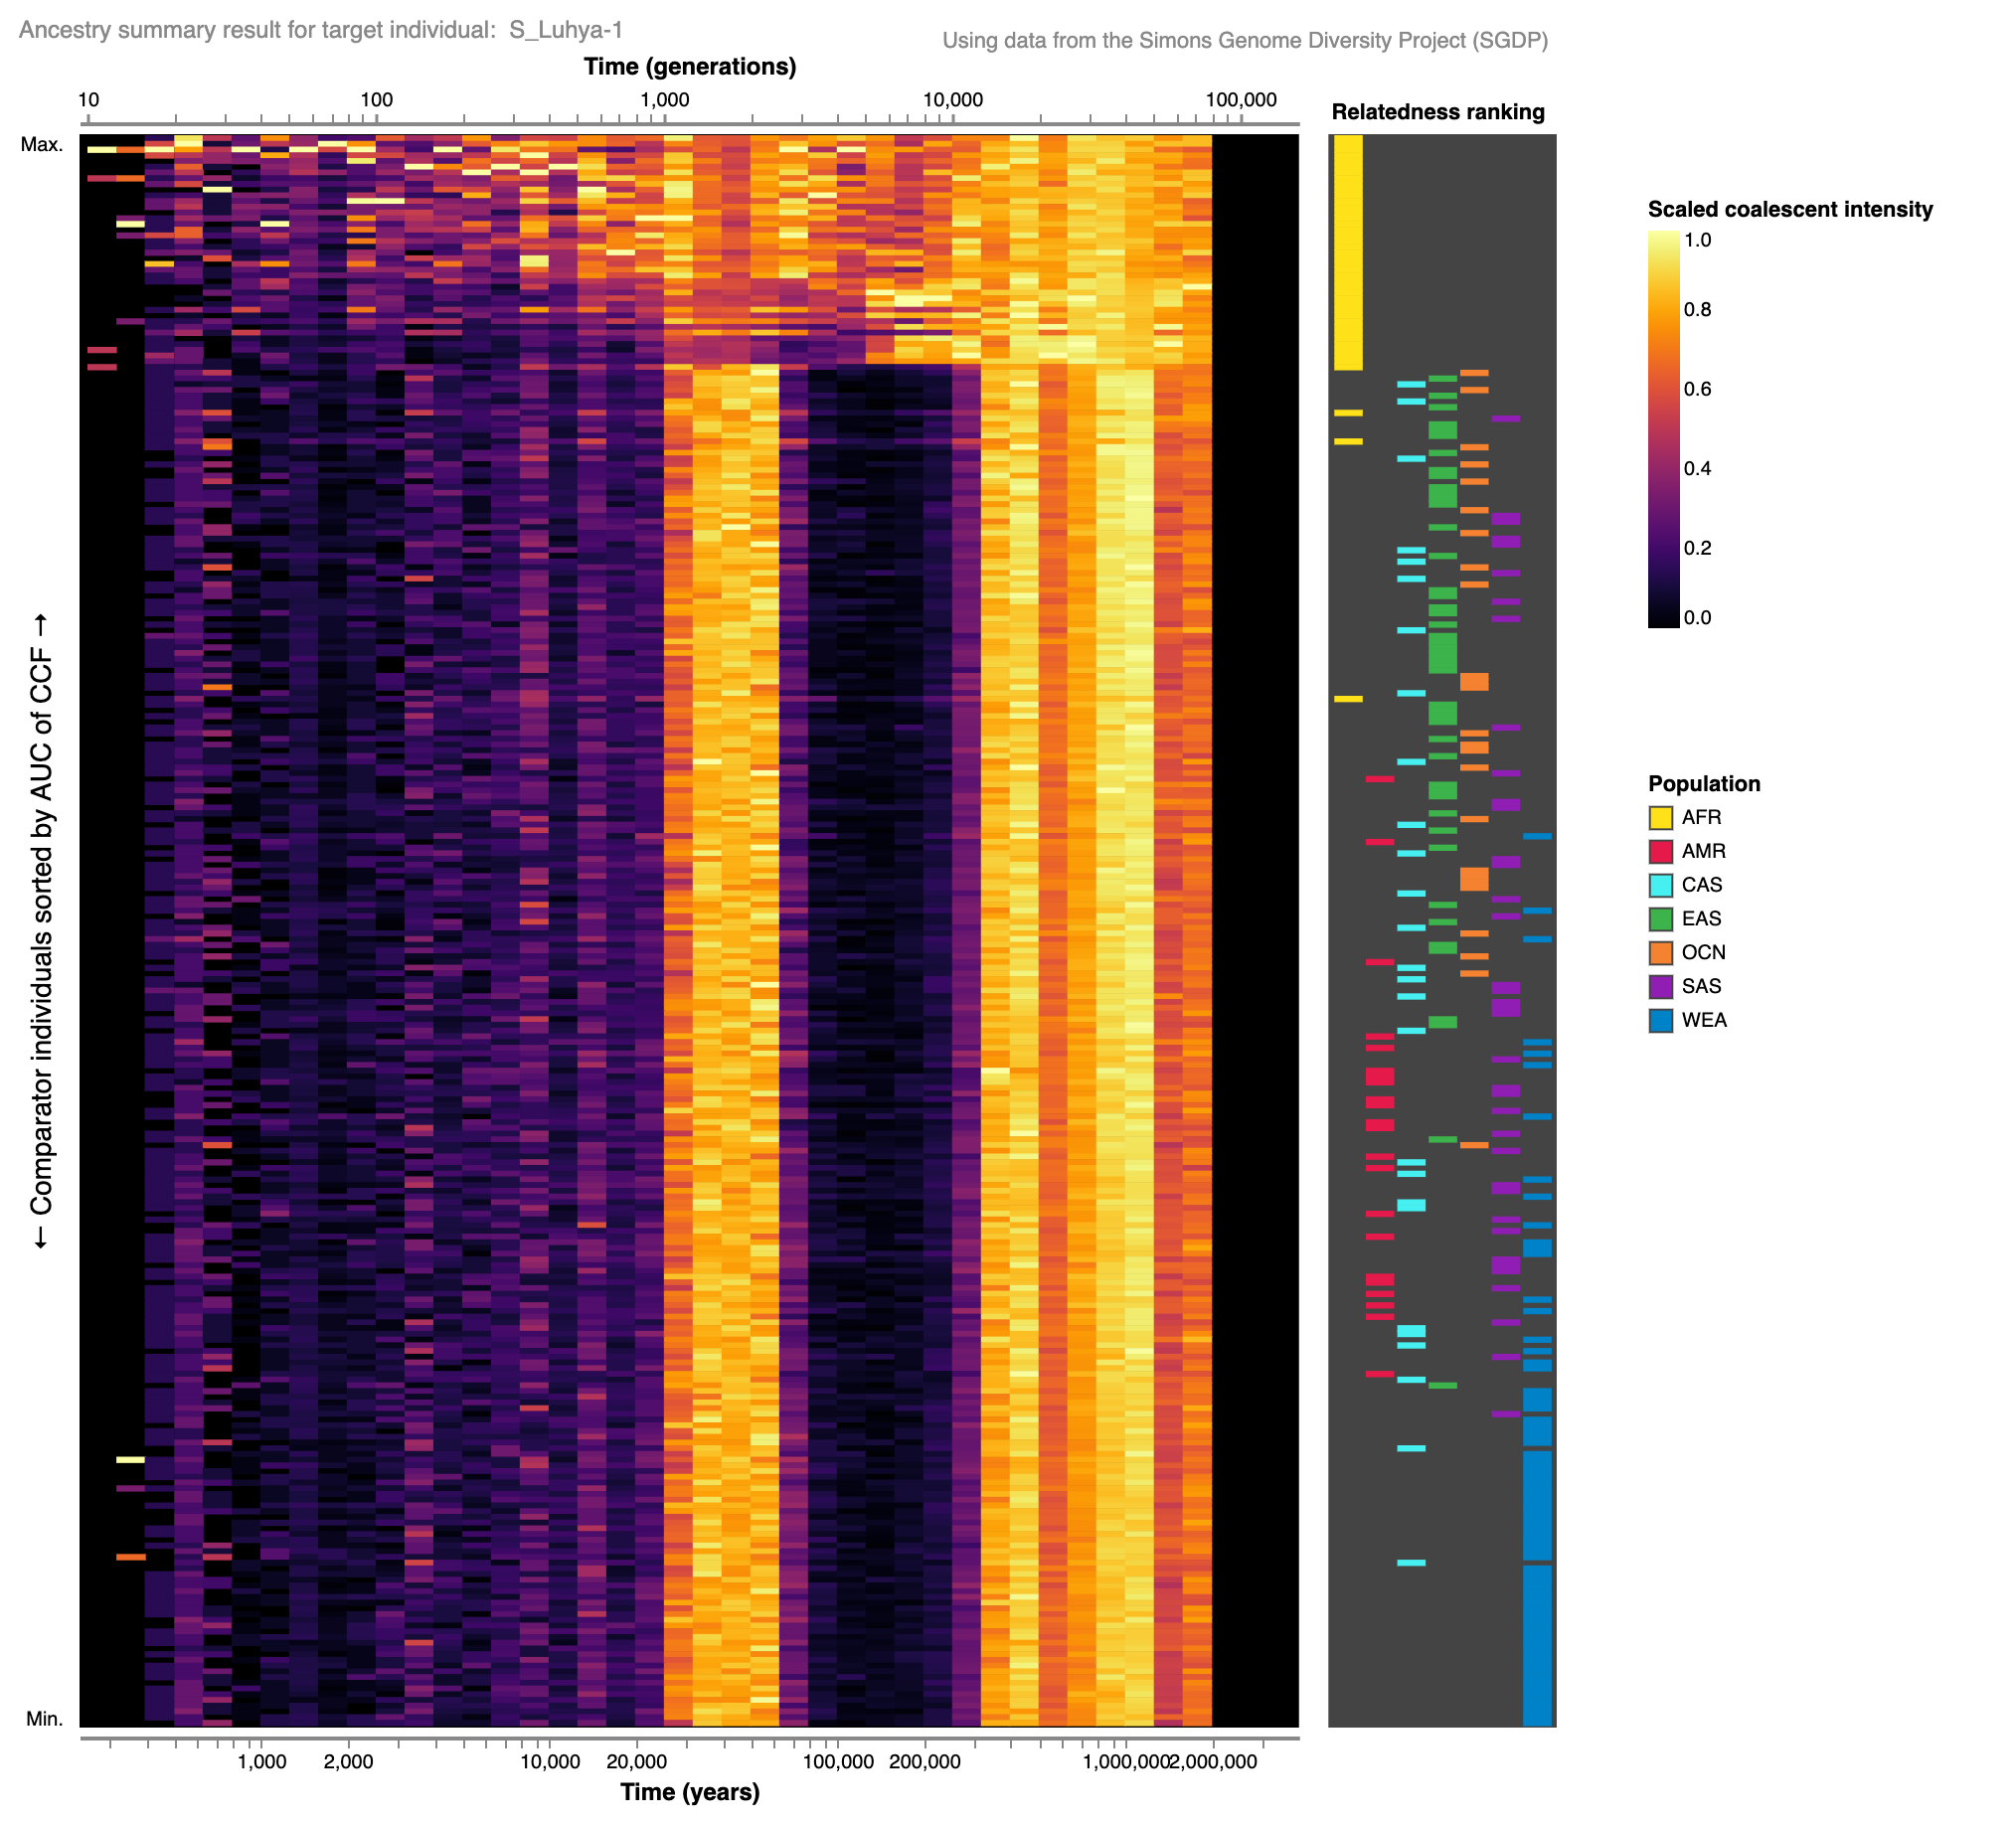
\includegraphics[width=0.5\textwidth]{plot/ch6/luhya}}%
	\caption{Inferred coalescent intensity function as calculated in \textcite{Albers2019} and exported from the web interface at \url{https://human.genome.dating/ancestry/} for Ju hoan North and Luhya individuals from the Simons Genome Diversity Panel. Shared coalescent intensity with other African individuals is found at the top of each figure within the yellow bar on the right hand side. }
	\end{figure}


The deep pre-history of Africa is poorly understood. Two populations are theorized to have diverged from the remainder of extant groups in the ancient past, though the actual timing of their divergences is contentious and similar to accepted estimates of the \gls{ooa} divergence $\sim$120kya \cite{Lipson2019}. The degree to which large-scale events such as this migration and other previously un-modelled events such as archaic introgressions (such as that observed by \textcite{Durvasula2019}) have contributed to inferred population structures is not well understood. The coalescent intensity function as proposed in \textcite{Albers2019}, for example, shows similarities between essentially all African groups including the San and \glspl{cahg} with regards to their coalescent histories around the time of our identified migration event. It is unlikely that this dip in coalescent intensity before the migration is due to mass population bottlenecks from super volcano activities, as was previously suspected \cite{Smith2018}. Populations identified here as receiving less genetic material from the migration (Khomani San, Ju Hoan, Mbuti, Biaka) show much attenuated coalescent intensity with other African populations between their supposed diversification and this migration. It is not clear how the San and other distantly related populations became recipients of a smaller amount of introgressed material. It is also not clear whether their differential acquisition of OoA genetic material may be sufficient to cause the entirety of African similarities before this period, implying a much larger role for population migrations in human history and explaining the significance of identifying a large portion of the genome as being derived from the migration. 

Much more work is needed to understand the place of this migration in African pre-history and to unravel the tangled web of deep relationships within the continent. 

\section{Better discrimination between closely related cell types with topic modelling}

Identifying shared groupings of active and accessible regulatory elements between closely related cell types is a difficult problem in functional genomics. It is especially relevant for cancers which have an unknown cell of origin, such as MLL-fusion driven leukemias. In Chapter 3, we adapt the cisTopic \gls{lda} model for the case of bulk ATAC-seq data. NGS data is becoming increasingly available, and large panels of celltype specific accessibility variation are available from large consortia such as \textcite{ENCODEProjectConsortium2012}. The approach, which we called \gls{blda}, uses a quantitative value for each peak region rather than a binary activity score as is appropriate for the single cell case. I demonstrate that the approach is superior to a naive implementation of cisTopic in several applications including pseudobulked data and a bespoke erythropoesis dataset. Though these comparisons are reassuring, and lend confidence to the results being generated, they do not constitute adequate benchmarking against gold-standard approaches. Identifying such approaches was difficult, as to our knowledge topic modelling has never been applied to bulk ATAC-seq data, and the closest class of approaches such as ChromHMM is not appropriate to answer the problems that we set out to address. This is true for two reasons. Firstly that chromHMM infers the most likely state of the genome but does not identify which states are statistically shared or distinct between different cell types. Secondly, because the performance of chromHMM to call distinct state paths in extremely closely related cell types (such as those studied in Chapter 4) is not well understood; extensions such as \textcite{Marco2017} are evaluated on datasets such as cell lines from the ENCODE project which are known to be extremely diverse. Explicit comparisons between these methods and their ability to identify differentially active regions (most directly assayed through simulation studies) should be performed to establish topic modelling as a viable approach for this class of problem.

Though empirically, our results are consistent with biological expectations, there remain many unanswered questions about the fine-scale details of the implementation. One such question is the choice of normalization method for read data, which has been shown to starkly impact the ability of peak-calling algorithms to identify enriched regions in ATAC-seq data \cite{Reske2020a}. We chose RPKM as a respected and reasonable first attempt, however experimentation is needed to determine the optimal method to compare amongst experiments from different centres and different protocols. This leads directly to the unanswered question of the effects of potential latent batch effects, for which I suggest a solution in the following paragraph. The inclusion of many cell types in analyses such as this necessarily increases the complexity of the topic model involved, however another unanswered question is the optimal granularity of a model for a specific purpose; is it better, for instance, to include all available cell types, or to select a few reasonable candidates for comparison? Part of the answer to this question lies in the number of topics that the model is able to reproducibly identify, which is a facet of these investigations not currently appreciated in the text mining literature. I suggest that reproduction of topics across many different stochastic inference instantiations may be a reliable way of increasing the signal to noise in key-word region identification. However, the methods for actually selecting the number of topics and hyper-parameter values were rudimentary in this thesis, and a more complete solution would involve inferring these values simultaneously with topic loadings. 

There have been many innovations in the field of topic modelling in recent years. The performance of \gls{blda} on pseudo-bulked and real data is encouraging, and encourages the use of improved methodologies with the ability to incorporate more data and address the issues raised above. One such class of model is hierarchical \gls{lda}, which is a simple extension of the LDA method that treats the number of topics as an unknown variable to be inferred along with topic loadings. The choice of $k$ for the applications in this thesis was highly non-trivial, and an automated procedure guaranteed to select a reasonable $k$ would be extremely beneficial for situations where the similarity structure of data is unknown. Additionally, structured topic models introduce the ability to intelligently learn associations between provided metadata and the probability of a topic occurring in a document. This has natural application to controlling for batch effects between disparate experimental sources as well as introducing prior information on the biological relationship of samples. This structured model would also be an ideal environment to combine ATAC-seq and DNAse-seq experiments while acknowledging and controlling for systematic differences. Another innovation can be drawn from the world of single cell analysis, where the ArchR pipeline choses to discard entirely the concept of peak regions of accessibility and instead works directly with a windowed view of the genome. This approach has the benefit of removing any ambiguity involved in estimating enriched regions and working directly with the underlying data, though at the cost of significant compute cost. For smaller analyses however, this may lead to more refined estimates of important regions, edge conditions notwithstanding. 

The BLDA method represents a preliminary attempt to use topic modelling for a difficult problem in functional genomics. The work in this thesis provides a foundation for further study into the potential for this kind of methodology in determining shared and distinct regulatory regions between similar cell types. 

\section{Novel Enhancers in MLL-AF4 Leukemia}

Despite recent progress in treatment options for childhood and infant leukemias, cancers driven by MLL translocations remain mostly incurable and show far worse outcomes than similar cancers without the MLL driver. In Chapter 4, I apply the BLDA method to a collection of ATAC-seq experiments from MLL-AF4 patients and cell lines alongside closely related healthy pre-proB (PPB) and proB (PB) cells. I show highly enriched topics consistently load onto the cancerous cells and that across stochastic replication they consistently contain a subset of associated regions for any threshold. ChIP-seq association shows that these regions are active enhancers in the MLL-AF4 patients, some of which have been previously annotated in distantly related cell types and some of which have not. I explore the relationship to other bound transcription factors such as RUNX1 and PAF1c in the discussion of Chapter 4. 

Due to the impacts of COVID, there are many aspects of this project which remain as future work. The first concerns computational analyses which I was unable to complete. These include full-scale analysis of the entirety of the ENCODE dataset and an in depth study of the identified regulatory patterns across cell types. Though this analysis would be of broad interest, it was never performed due to the weeks-long runtimes required. The second concerns experimental validation. In order to pursue these associations, capture-C experiments must identify first which promoters are interacting with these enhancers in these particular cell types. Additionally, if a sufficiently encouraging pathway involving these enhancers can be identified, experimental deletion can identify if their presence is necessary for leukemogenesis. One interesting pathway for experimental validation with clinical applications concerns the possibility that these enhancer elements represent a DOT1L rescue pathway. It has been previously shown that DOT1L inhibition is not sufficient to eliminate leukemia blasts in vitro, despite strong interaction between the fusion protein and the DOT1L protein and a proven subset of enhancers whose promoter interactions are dependant on H3K79me2. The enhancers identified in this thesis appear to be statistically depleted for H3K79me2, indicating that DOT1L is not necessary for their function. In order to study their use in a putative DOT1L rescue pathway, their accessibility should be assayed before and after treatment with a DOT1L inhibitor such as EPZ-5676. This would demonstrate their utility and motivate further study in possibly novel mechanisms of action in this leukemia. One interesting possibility is that the enhancer regions are being recruited not by the fusion protein but by wild-type MLL. This is suggested by the ChIP-seq associations, which show high enrichment of MLL binding at these sites without any enrichment for the fusion protein C terminus AF4. Though it is possible, and indeed likely, that this difference is due to inefficient antibodies for AF4 pulldown, the independent action of the wildtype MLL protein on the regulatory landscape of cancer cells represents an interesting possibility for further study, especially as the binding sites of the fusion protein are typically seen to represent a subset of the binding sites of the wild-type protein.

Overall this analysis represents an initial investigation of distinct regulatory elements in MLL-AF4 patients. I used the BLDA method to nominate potential regions and used external data to show that they are functional within this cellular context. These regions represent strong candidates for functional validation. Furthermore, this analysis demonstrates the potential of the BLDA method to identify distinct and interesting regulatory regions in extremely similar cell types.

\section{Concluding Remarks}

This thesis has introduced, developed, and applied new methods for the analysis of next generation sequencing data. Two different problems are approached through the lens of machine learning. The first method, SMC2, represents an algorithmic implementation of an intricately designed statistical model with decades of motivation in population genetics. Despite this, our results demonstrate that large-scale events can be missed by conventional analyses which fail to fully parameterize migration. The second method, BLDA, represents an incremental upgrade on a general method which contains no deep relationship to the biology which it models, yet still yields actionable insights into the pathology of an incurable leukemia. The diversity of approaches here demonstrated show the potential for machine learning algorithms of all kinds in this growing field.  






% mll

% experimental follow up 
% mix of some novel enhancers and ones which are already annotated in different cell types. 
% 	this is probably the most likely scenario, but also provides some insight into the possible mechanisms and pathways that are triggered by the fusion protein. 

% Analyses that I wish I did but didn't do due to time
%	whole ENCODE
% 	corces + erythropoiesis 
% 	more thorough comparisons with chromHMM based segmentation models 




% blda 

% the approach is valid for any closely related cell types 
% 	this is extremely difficult in practice. Thgins like chromHMM work in some situations but are almost always evaluated against cell types which have hugely different regulatory grammar (ex the diHMM appraoch is evaluated on the ENCODE cell lines.)
% don't us peak regions, just use all regions such as archR

% The adaptations made to the cistopic model are minimal, and there are many questions that remain to be answererd
% 	which normalisation method is the most suitable
%	what effect does batch have on this? are we seeing things due to batches?
%	what is the optimal granularity and the best way to find the numbers of topics and keyword regions for analysis? 


% methodological extensions
% hierarchical LDA for deciding the correct number of topics (and alpha/beta parameters), essentially combining these parameters into the inference procedure
% 	structured text modelling incorporating metadata about the things. these include things liek patients age or disease status, batch effects  
%	topic model of all relevant things together (including the chip-seq). LDA-dual model can do this for ChIP-seq and ATAC-seq per document



% mll







% The back migration
% 	As explained in the discussion section of the chapter, this is not an unprecedented find but it is novel to be found in the somatic genome, which has allowed us to estimate its magnitude for the first time
% 	interestingly, the finding has already been replicated twice using new generation DL approaches. we expect it to be identified by any algorithm which explicitly parameterises directional migration 
% 	the interpretation in terms of population structure of Africa is interesting, and begs the question of how far this trend might actually extend. as an example, the KhoeSan are thought to be the most distnatly related population on the continent, but could this in fact just be due to their relative lack of involvement in this migration, leading to a substnatital difference between them and the other Africans?
% clearly population structure on the continent is extremely 






% \subsection{The Ancestral Recombination Graph (ARG) and admixture inference in the ancient past}


% The phylogenetic trees over a set of samples as they change along the genome through recombination, collectively referred to as the ancestral recombination graph (ARG) \cite{Griffiths1997a,Rasmussen2014}, record all information about the samples' evolutionary history.  This history itself is shaped by the population's demography, a statistical relationship that is quantified by the coalescent-with-recombination (CwR) model \cite{Griffiths1997a}.  The ARG is a complex data structure which is only weakly constrained by the observed genetic polymorphisms, making inference of demography difficult. By making approximations to the CwR, for instance by making an independent-sites assumption, efficient parametric inference of demography becomes possible \cite{Excoffier2013,McVean2005}.  Methods including {\tt PSMC} \cite{Li2011}, {\tt diCal} \cite{Steinrucken2015} and {\tt SMC++} \cite{Terhorst2015} allow non-parametric inference of demography under a closer approximation to the CwR, but one that does not include gene flow between populations. MSMC \cite{Schiffels2014} introduced the cross-coalescent rate and {\tt MSMC-IM} described how to interpret this rate in the context of a isolation-migration model to estimate a migration rate between populations\cite{Wang2019a}. However, these methods are not well suited for estimating directional migration rates. 

% Here we extend SMCSMC (Sequential Monte Carlo inference of the Sequentially Markovian Coalescent, \cite{Henderson2018}) to allow inference of directional migration.  SMCSMC is a Bayesian method that uses a particle filter to explicitly sample from the posterior distribution of ARGs over multiple diploid samples under the full CwR model.
% Since particle filters operate by simulating latent variables (here the ARG) under the statistical model of interest, it becomes possible to handle complex demographic scenarios.  We exploit this by extending the CwR model to include time-varying directional migration rates in a two-island demographic model.  We use the posterior sample of ARGs including migration events to update the parameters of the demographic model, using either expectation-maximization or a variational Bayes procedure, and iterate these steps until convergence.   We apply SMCSMC to estimate directional migration rates in whole genome sequencing data from the Simons Genome Diversity Panel (SGDP) \cite{Mallick2016} and the Human Genome Diversity Panel (HGDP) \cite{Bergstrom2019} to investigate population structure around the OoA event.

% \subsection{Migration initialisation Values} \label{ch2:initial}

% We select a more comprehensive set of initiation pardameters and particle values and use them to analyze a Yoruban and French individual from SGDP (Fig \ref{init_yri}). The effect of the initial migration rate seems relatively consistent for low values (0.5 - 2.0),while an increasingly small migration peak is seen for higher initial magnitudes 4.0 - 10.0. Again, beginning with an initial rate of zero tends to lead to highly unstable estimates of effective population size and migration rates. For the remainder of the analyses in this article, we choose to use an initial rate of 1.0. 



% \begin{figure}
% 	\centering
% 	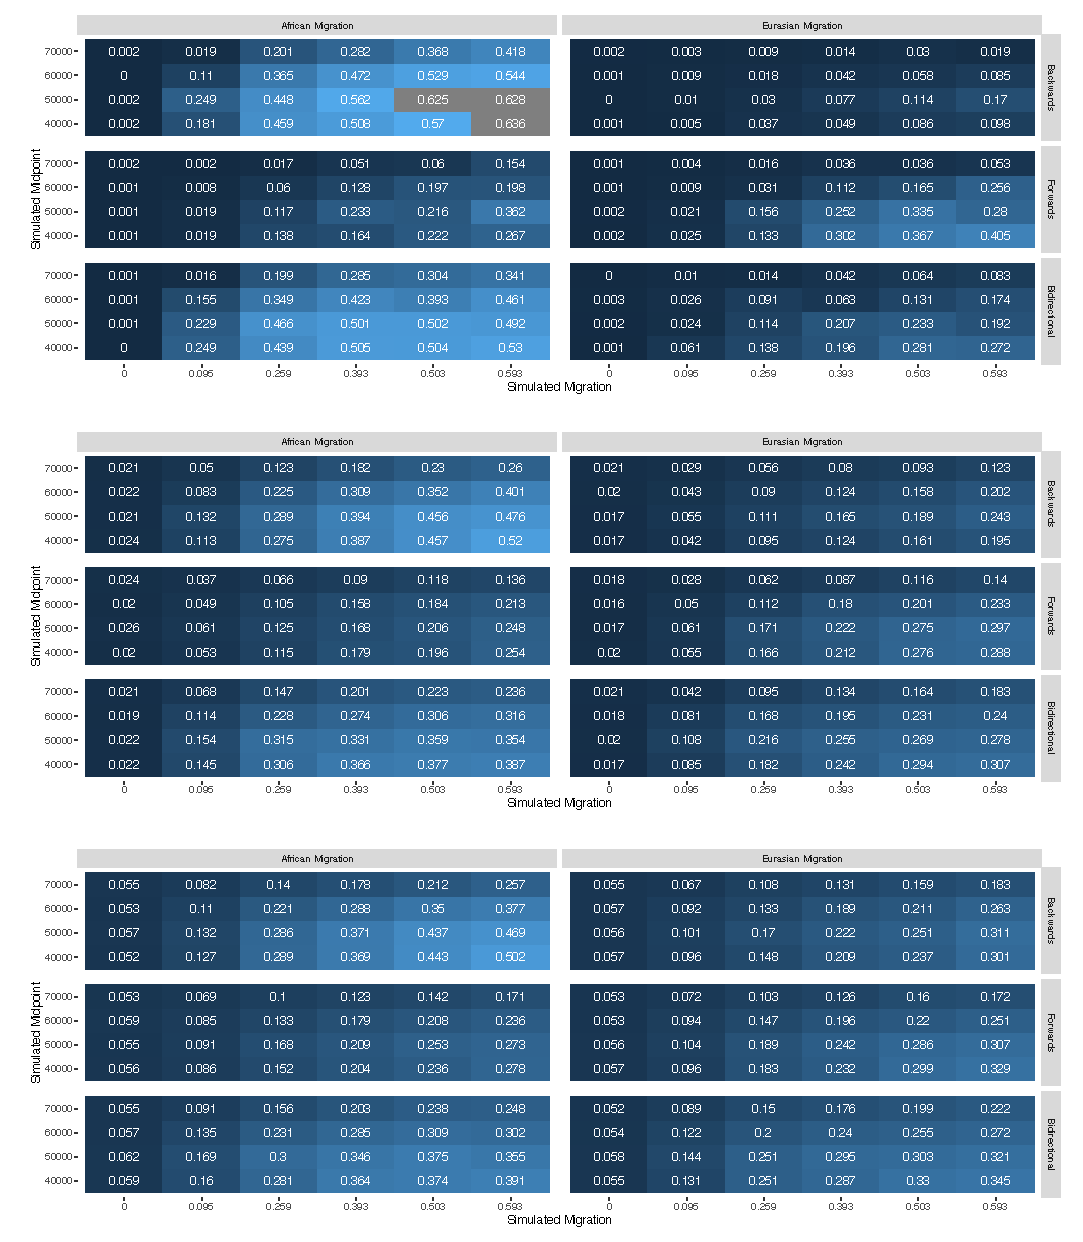
\includegraphics[width=\textwidth]{plot/all_integrated_sims.pdf}
% 	\caption[Integrated migration for three cases of simulated demographies]{ {\bf Integrated migration fraction (IMF) in the last 100ky for three cases of simulated demography shown in \ref{fig:backsim}, \ref{fig:bisim}, and \ref{fig:fwdsim}.} Simulations were performed as per Supplemental Section \ref{methods:simproc} with an additional parameter for the initial migration rate used to initialise the SMCSMC particle filter. The timing and IMF simulated are as per the aforementioned figures. From top to bottom, inference was initiated with 0, 1, and 5 4$N_0$ population replacement per generation in the specified direction (backwards, bidirectionally, and forwards).}
% 	\label{fig:intsim}
% \end{figure}

% \begin{figure}
% 	\centering
% 	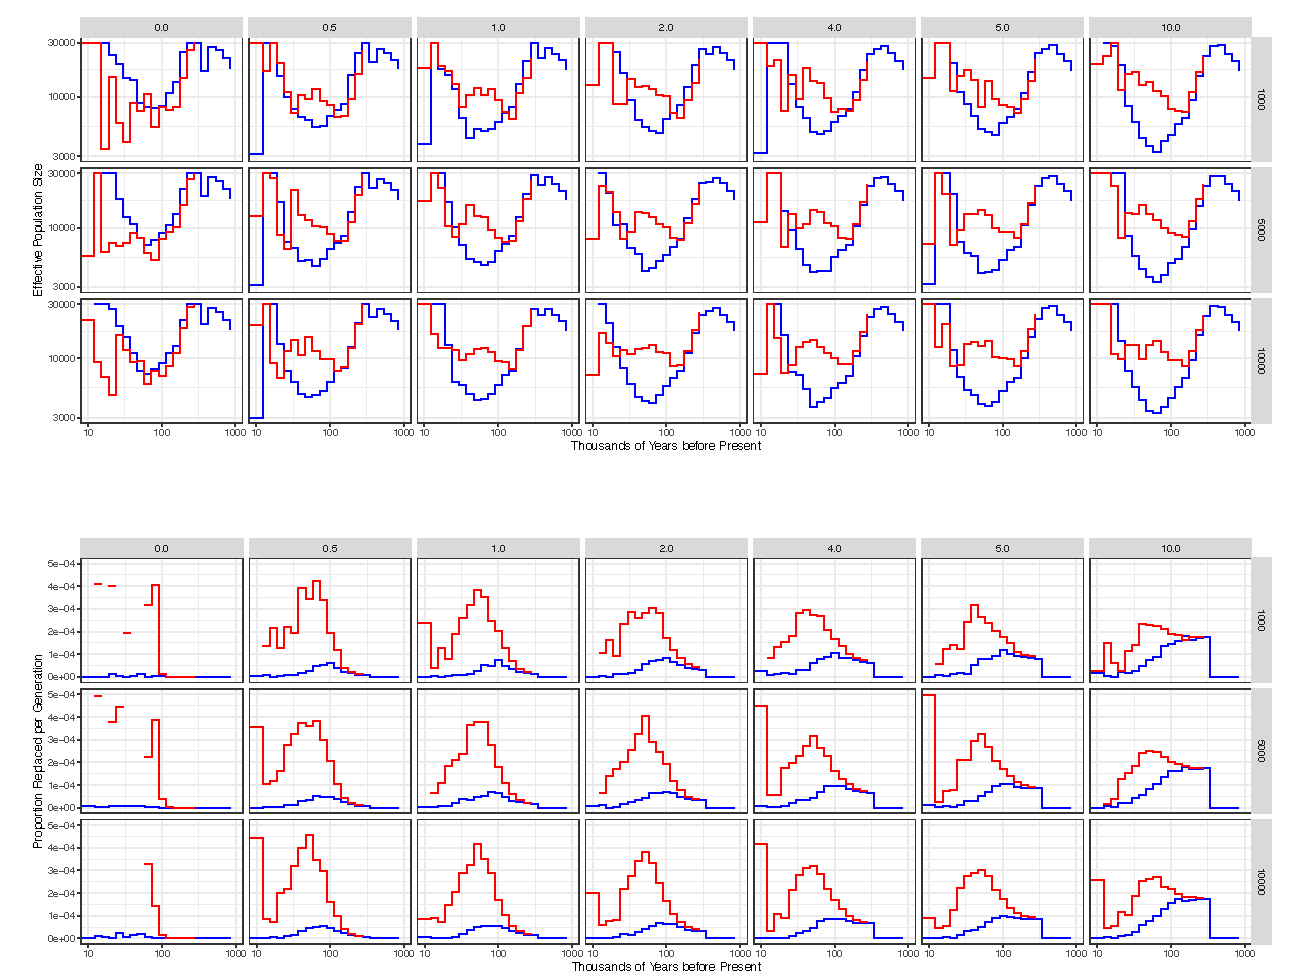
\includegraphics[width=\textwidth]{plot/yri_dif_migs.pdf}
% 	\caption[The effect of initial mirgation on demographic inference]{ {\bf The effect of initial migration parameter on demographic inference.} Effective population size and migration history of a Yoruban ({\tt S\_Yoruba-1}) and a French ({\tt S\_French-1}) individual from the Simons Genome Diversity panel were modelled with SMCSMC. The initial migration proportion, in units of 4 $N_0$ proportion of the population replaced per generation was varied along the X axis, while the number of particles is varied along the Y. 10 iterations of variational Bayes was used for parameter inference, while 5000 particles were used infer the ancestral recombination graph.}
% 	\label{fig:init_yri}
% \end{figure}

% \minitoc

